\section{Video Prediction for Control}

\begin{figure}[t]
    \centering
    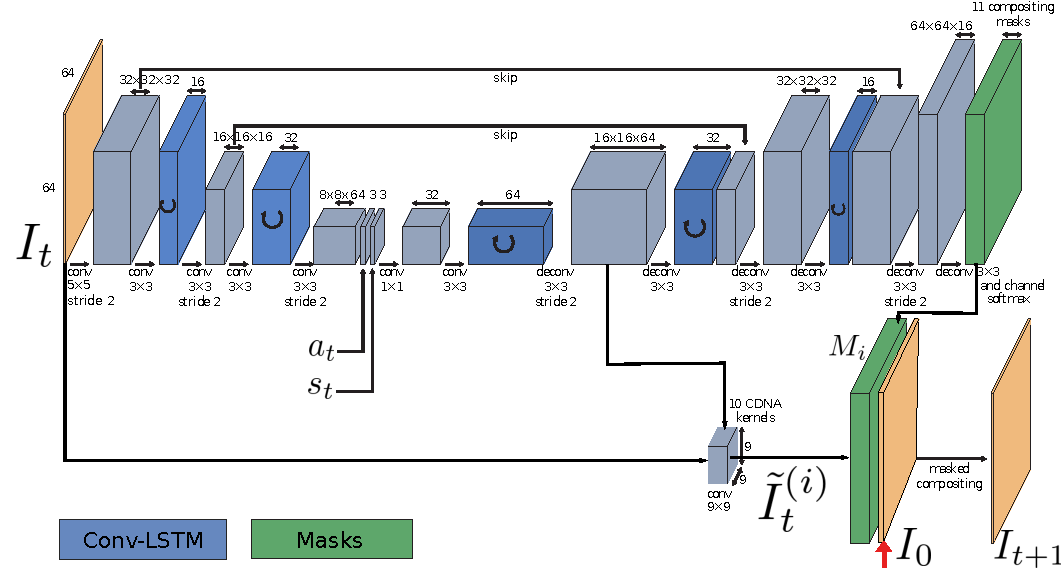
\includegraphics[width=\columnwidth]{images_sna/occlusionaware/occlusion_model.pdf}
    \caption{\small{Simplified SNA model based on \autoref{eqn:simplemodel}. The red arrow indicates where the image from the first time step $I_0$ is concatenated with the transformed images $\tilde{I}^{(i)}_t$ multiplying each channel with a separate mask to produce the predicted frame for step $t+1$. \todo{add appflow} }}      \label{fig:occlusion_model}
\end{figure}

\subsection{Video Prediction via Pixel Transformations}
\label{sec:model}
Visual MPC requires a model that can effectively predict the motion of the selected pixels $\pixel_0^{(1)}, \dots, \pixel_0^{(P)}$ up to $T$ steps into the future (except for the classifier-based cost function described in section \ref{subsec:class_cost}).
In this work, we extend the model proposed in \cite{finn_nips}, where this flow prediction capability emerges implicitly, and therefore no external pixel motion supervision is required. Future images are generated by transforming past observations. The model uses stacked convolutional LSTMs that predict a collection of pixel transformations at each time step, with corresponding composition masks. In this model, the previous image $I_t$ is transformed by $N$ separate transformations, and all of the transformed images $\tilde{I}_t^{(i)}$ are composited together according to weights obtained from the predicted masks. Intuitively, each transformation corresponds to the motion of a different object in the scene, and each mask corresponds to the spatial extents of that object. Let us denote the $N$ transformed images as $\tilde{I}_t^{(1)}, ..., \tilde{I}_t^{(N)}$, and the predicted masks as $\mathbf{M}_1, ...\mathbf{M}_N$, where each 1-channel mask is the same size as the image. The next image prediction is then computed by compositing the images together using the masks: $\hat{I}_{t+1} = \sum_{i=1}^N \tilde{I}_t^{(i)} \mathbf{M}_i$. To predict multiple time steps into the future, the model is applied recursively. These transformations can be implemented as warping using a flow-field that defines the positions for bilinear sampling in the image. (Previous versions used convolution kernels to transform images). The warping transformations can be interpreted as a stochastic transition operator allowing us to make probabilistic predictions about future locations of individual pixels. To predict the future positions of the designated pixels $d^{(i)}$, the same transformations which are used for the images are applied to $P_{t,d^{(i)}}$ such that $P_{t+1,d^{(i)}} = \frac{1}{P_s}\sum_{i=1}^N \tilde P^{(i)}_{t,d^{(i)}} \mathbf{M}_i $, where $\frac{1}{P_s}$ is a normalizing constant to ensure that $P_{t+1,d^{(i)}}$ adds up to 1 over the spatial dimension of the image. Since this prior model predicts images only based the previous image, it is unable to recover shapes (e.g. objects) after they have been occluded, for example by the robot arm. Therefore, this model is only suitable for planning motions where the user-selected pixels are not occluded during the manipulation, which restricts its use in cluttered environments or with multiple selected pixels. In the next section, we discuss our proposed occlusion-aware model, which lifts this limitation by employing temporal skip connections.

\subsection{Skip Connection Neural Advection Model}

\begin{figure}[t]
        \centering
        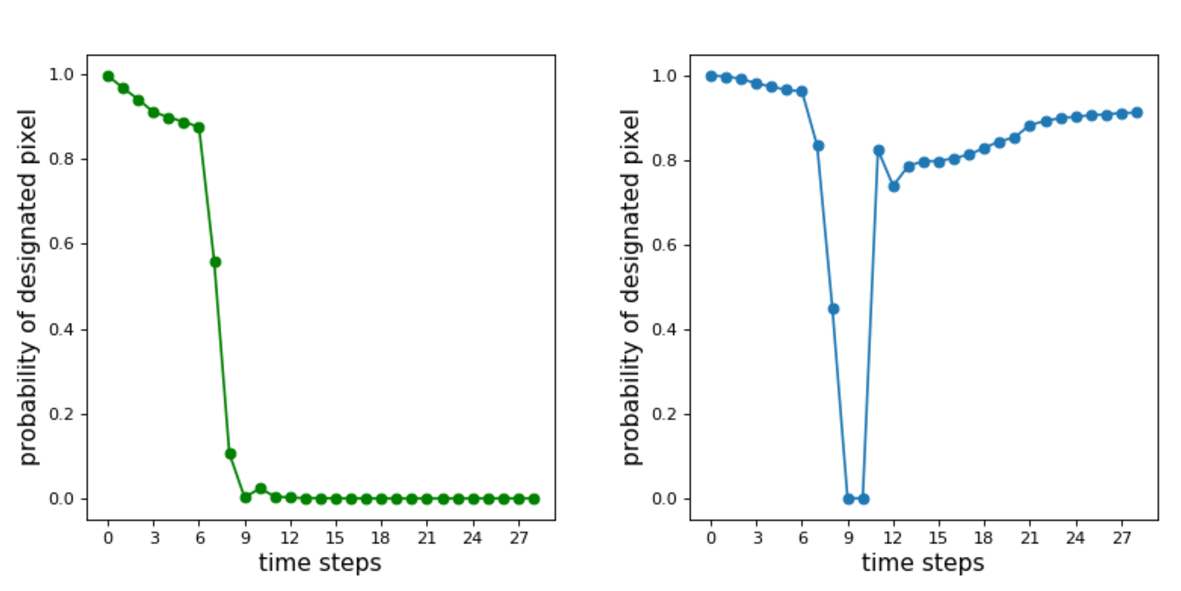
\includegraphics[width=0.9\columnwidth]{images_sna/occlusionaware/probability_curves.pdf}
        \caption{Predicted probability $P_{d^{(0)}}(t)$ of the designated pixel being at the location of the blue dot indicated in \autoref{fig:desig_pix_bluedot} for the DNA model (left) and the SNA model (right).}        \label{fig:pix_reqppear_graph}
\end{figure}

\label{sec:occlusion_model}
To enable effective tracking of objects through occlusions, we propose an extension to the video-prediction model proposed in~\cite{finn_nips} that incorporates temporal skip connections. 
\begin{wrapfigure}{r}{.37\columnwidth}
% \vspace{-0.6in}
        \centering
        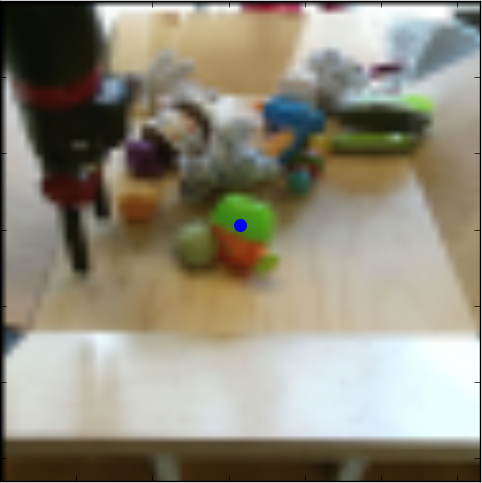
\includegraphics[width=0.4\columnwidth]{images_sna/occlusionaware/img_desigpixb0.png}
        \caption{The blue dot indicates the designated pixel}
        \label{fig:desig_pix_bluedot}
% \vspace{-1in}
\end{wrapfigure}
This model uses a similar multilayer convolutional LSTM structure; with the crucial difference that the transformations now allow transforming pixels not only from the previous but from \emph{all} previous images $I_0,...I_{t}$. Transforming from all previous images comes with increased computational cost. However we found that in practice a greatly simplified version of this model, where transformations are applied only to the previous image and the \emph{first image} of the sequence. We will therefore first present the generic model, and then describe the practical simplifications. We refer to this model as the skip connection neural advection model (SNA), since it handles occlusions by copying pixels from prior images in the history such that when a pixel is occluded (e.g., by the robot arm or by another object) it can still reappear later in the sequence. When predicting the next image $\hat{I}_{t+1}$, the generic SNA model transforms each image in the history according to a different transformation and with different masks to produce $\hat{I}_{t+1}$ (see \autoref{fig:general_model} in the appendix):

\begin{equation}
\hat{I}_{t+1} =  \sum_{j=t-T}^{t} \sum_{i=1}^{N} \mathbf{M}_{i,j} \tilde{I}_{j}^{(i)}
\label{eqn:general_model}
\end{equation}
In the case where $t < T$, negative values of $j$ simply reuse the first image in the sequence. This generic formulation can be computationally expensive, since the number of masks and transformations scales with $T \times N$. A more tractable model, which we found works comparably well in practice in our robotic manipulation setting, assumes that occluded objects are static throughout the prediction horizon. This assumption allows us to dispense the intermediate transformations and only provide a skip connection from the very first image in the sequence, which is also the only real image, since all of the subsequent images are predicted by the model:
\begin{equation}
\hat{I}_{t+1} =  I_0 \mathbf{M}_{N+1} +  \sum_{i=1}^{N} \tilde{I}_t^{(i)} \mathbf{M}_i
\label{eqn:simplemodel}
\end{equation}
This model only needs to output $N+1$ masks. We observed similar prediction performance when using the original image $I_0$ instead of the transformed image $\tilde{I}_0$ and therefore use the simplified model in \autoref{eqn:simplemodel} in all of our experiments. We provide an example of the model recovering from occlusion in \autoref{fig:pix_reappear}. In the figure, the arm moves in front of the designated pixel, marked in blue in \autoref{fig:desig_pix_bluedot}. The graphs in \autoref{fig:pix_reqppear_graph} show the predicted probability of the designated pixel, which is stationary during the entire motion, being at its original position at each step. Precisely when the arm occludes the designated pixel, the pixel's probability of being at this point decreases. This indicates that the model is `unsure' where this pixel is. When the arm unoccludes the designated pixel, it should become visible again, and the probability of the designated pixel being at its original position should go up. In the case of the DNA model and its variants~\cite{finn_nips}, the probability mass does not increase after the object reappears. This is because the DNA model cannot recover information about object that it has `overwritten' during its predictions.



Consequently these models give wrong predictions when the designated pixel becomes occluded often causing the model to predict that the pixel \emph{moves with the arm}. We identified this as one of the major causes of planning failure when using these prior models. By contrast our SNA model predicts that the occluded object will not move, which is indicated by a sharp increase in the probability value evaluated at the original position of the pixel after becoming unoccluded (see \autoref{fig:pix_reqppear_graph}).

\begin{figure}
    \centering
    \begin{subfigure}{0.9\columnwidth}
    \centering
        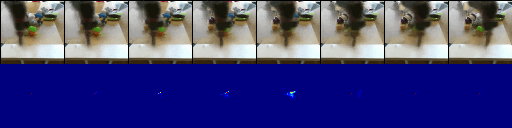
\includegraphics[width=1.\linewidth]{images_sna/occlusionaware/cdna_1ststep_bckgd_gen_pixb0_overtime.png}
        \caption{Skip connection neural advection (SNA) does not erase or move objects in the background}
        \label{fig:Ng1}
    \end{subfigure}
    \begin{subfigure}{0.9\columnwidth}
    \centering
        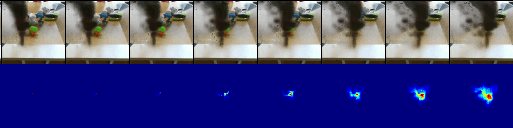
\includegraphics[width=1.0\linewidth]{images_sna/occlusionaware/orig_dna_gen_pixb0_overtime.png}
        \caption{Standard DNA \cite{foresight} exhibits undesirable movement of the distribution $P_{d}(t)$ and erases the background}
        \label{fig:pix_reappear}
    \end{subfigure}
    \caption{
    %\protect\subref{fig:Ng1} 
    Top rows: Predicted images of arm moving \textit{in front of} green object with designated pixel (as indicated in \autoref{fig:desig_pix_bluedot}). 
    %(\protect\subref{fig:Ng2}) 
    Bottom rows: Predicted probability distributions $P_{d}(t)$ of designated pixel obtained by repeatedly applying transformations.}
    \label{fig:pix_reappear}
\end{figure}
